\documentclass{article}

\usepackage{amsmath, amsthm, amssymb}
\usepackage{geometry}
\geometry{margin = 3.0 cm}
\usepackage{float}
\usepackage{algorithm2e}
\usepackage{caption}
\usepackage[]{mcode}
\usepackage{algpseudocode}
\algblockdefx[NAME]{Input}{EndInput}
    [1][]{\textbf{Input:} #1}
    {}

\algblockdefx[NAME]{Output}{EndOutput}
    [1][]{\textbf{Output:} #1}
    {}

\newcommand{\myalg}[2]{\begin{figure}[h]
    { \renewcommand{\figurename}{Algorithm}
\begin{center}
\begin{minipage}{0.6\textwidth}
\hrulefill
\begin{algorithmic}[1]
    #1
\end{algorithmic}
\hrulefill
\end{minipage}
\end{center}
\caption{#2}
}
\end{figure}}

\renewcommand{\l}{\lambda}
\renewcommand{\L}{\Lambda}
\renewcommand{\mod}{~\mathrm{mod}~}
\renewcommand{\div}{~\mathrm{div}~} 
\renewcommand{\vec}[1]{\mathbf{#1}}

\renewcommand{\(}{\left(}
\renewcommand{\)}{\right)}

\newcommand{\dist}{\text{dist}}

\newcommand{\mat}[1]{\begin{pmatrix} #1 \end{pmatrix}}
\newcommand{\room}{\hspace{0.5cm}}
\newcommand{\hl}[1]{\textbf{#1}}
\newcommand{\ceil}[1]{\lceil #1 \rceil}
\newcommand{\floor}[1]{\lfloor #1 \rfloor}
\newcommand{\var}[1]{$\mathtt{#1}$}
\newcommand{\mc}[1]{\mathcal{#1}}
\newcommand{\hot}[1]{\mathcal{O}\(#1\)}
\newcommand{\minimx}[4]{\begin{pmatrix}{#1} & {#2} \\ {#3} & {#4} \end{pmatrix}}

\newcommand{\uin}{u_i^n}
\newcommand{\uinp}{u_i^{n+1}}
\newcommand{\uinm}{u_i^{n-1}}
\newcommand{\uipn}{u_{i+1}^n}
\newcommand{\uimn}{u_{i-1}^n}
\newcommand{\uimnp}{u_{i-1}^{n+1}}
\newcommand{\uipnm}{u_{i+1}^{n-1}}
\newcommand{\uipnp}{u_{i+1}^{n+1}}

\newcommand{\ujn}{u_j^n}
\newcommand{\ujnp}{u_j^{n+1}}
\newcommand{\ujnm}{u_j^{n-1}}
\newcommand{\ujpn}{u_{j+1}^n}
\newcommand{\ujmn}{u_{j-1}^n}
\newcommand{\ujmnp}{u_{j-1}^{n+1}}
\newcommand{\ujpnm}{u_{j+1}^{n-1}}
\newcommand{\ujpnp}{u_{j+1}^{n+1}}

\newcommand{\xin}[1]{{#1}_{i}^n}
\newcommand{\xinp}[1]{{#1}_{t i}^{n+1}}
\newcommand{\xtinm}[1]{{#1}_{t i}^{n-1}}
\newcommand{\xipn}[1]{{#1}_{t i+1}^n}
\newcommand{\ximn}[1]{{#1}_{t i-1}^n}
\newcommand{\ximnp}[1]{{#1}_{t i-1}^{n+1}}
\newcommand{\xipnm}[1]{{#1}_{t i+1}^{n-1}}
\newcommand{\xipnp}[1]{{#1}_{t i+1}^{n+1}}

\newcommand{\yin}[1]{{#1}_{i}^n}
\newcommand{\yinp}[1]{{#1}_{i}^{n+1}}
\newcommand{\ytinm}[1]{{#1}_{i}^{n-1}}
\newcommand{\yipn}[1]{{#1}_{i+1}^n}
\newcommand{\yimn}[1]{{#1}_{i-1}^n}
\newcommand{\yimnp}[1]{{#1}_{i-1}^{n+1}}
\newcommand{\yipnm}[1]{{#1}_{i+1}^{n-1}}
\newcommand{\yipnp}[1]{{#1}_{i+1}^{n+1}}

\newcommand{\vin}{v_i^n}
\newcommand{\vinp}{v_i^{n+1}}
\newcommand{\vinm}{v_i^{n-1}}
\newcommand{\vipn}{v_{i+1}^n}
\newcommand{\vimn}{v_{i-1}^n}
\newcommand{\vimnp}{v_{i-1}^{n+1}}
\newcommand{\vipnm}{v_{i+1}^{n-1}}
\newcommand{\vipnp}{v_{i+1}^{n+1}}

\newcommand{\dt}{\Delta t}
\newcommand{\dx}{\Delta x}
\newcommand{\dxi}{\Delta \xi}
\newcommand{\ctx}{\frac{c\dt}{\dx}}
\newcommand{\half}[1]{\frac{{#1}}{2}}




\newtheorem{lem}{Lemma}

\usepackage{tikz} \usetikzlibrary{shapes}
\usetikzlibrary{arrows}

\tikzset{node distance=3cm, auto}

\begin{document}
\title{Exercise F4a}
\author{Abe Wits (3629538)}
\date{2015/06/05}

\maketitle

\setlength{\parskip}{0.2 cm}
\setlength{\parindent}{0.0 cm}

\section*{Write models 1 and 2 as a system of two first-order PDEs (in time) as discussed in exercise \textbf{SC1}}
We can rewrite $u_{tt} = u_{xxx}$ as;
$$
\begin{cases}
v = u_t\\
v_t = u_{xxx}
\end{cases}
$$

\section*{Describe and implement a boundary-value (BV) technique for both models. For a description of BV we refer to the documents on the web page of this course. Note that different choices can be made for the time-integration part of BV and also for its (extra) final condition at $t=T$}
We have to make our PDEs discrete. We use leapfrog for our time integration and we use the $\hot{(\dx)^2}$ space discretization we derived in SC1;
$$u_t \approx \frac{\uinp - \uinm}{2\dt} \;\;\;\;\mathrm{and}\;\;\;\;v_t \approx \frac{\vinp - \vinm}{2\dt}$$
$$u_{xxx} \approx \frac{-\half{u_{i-2}^n}+\uimn-\uipn+\half{u_{i+2}^n}}{(\dx)^3}$$

We want to construct a system of linear equations that solves our PDE. The equations above can be used to construct linear constraints: we want to enforce that $v=u_t$ and $v_t=u_{xxx}$;
$$v = u_t \approx \frac{\uinp - \uinm}{2\dt}$$
\begin{equation}
\uinp-2\dt\vin-\uinm = 0
\label{eq:uin}
\end{equation}
And similarly:
$$\frac{\vinp - \vinm}{2\dt} \approx v_t = u_{xxx} \approx \frac{-\half{u_{i-2}^n}+\uimn-\uipn+\half{u_{i+2}^n}}{(\dx)^3}$$
\begin{equation}
\vinp-\frac{2\dt}{(\dx)^3}\(-\half{u_{i-2}^n}+\uimn-\uipn+\half{u_{i+2}^n}\)-\vinm = 0
\label{eq:vin}
\end{equation}
In this system we see $\uin$ and $\vin$ as our variables. Let $T = N\dt$, then $n\in\{0,1,\dots,N\}$. Similarly we choose $x_M=x_{max}$ and $x_0=x_{min}$, with $m \in \{0,1,\dots,M-1\}$. We will handle boundary conditions in the space direction and our choice of $\dx$ separately for the different models.
Notice that our constraints are invalid if they contain non-existent variables such as $u_i^{N+1}$, $v_i^{N+1}$, $u_i^{-1}$ or $v_i^{-1}$. We do not use such invalid constraints, but add boundary conditions for $n=0$ and $n=N$ instead:
\begin{equation}
u_i^0 = u(x_i, 0)
\label{eq:ui0}
\end{equation}
\begin{equation}
u_i^N = u(x_i, T)
\label{eq:uiN}
\end{equation}
\begin{equation}
v_i^0 = v(x_i, 0)
\label{eq:vi0}
\end{equation}
\begin{equation}
v_i^N = v(x_i, T)
\label{eq:viN}
\end{equation}
The functions $u_0$, $v_0$ (the initial conditions)  and $u_T$, $v_T$ (the final conditions) are different functions for model 1 and model 2.
If all boundary conditions are chosen correctly, the number of constraints is exactly equal to the number of variables. We will write the system in the standard form, $A w = b$, where $A$ is a (known) matrix with all constraints, $b$ is a (known) vector with all the constants from the constraints, and $w$ the (unknown) vector that will contain our solution.

Let $w=(w^0, w^1, \dots w^N)^T$, where $w^n=(w_0^n,w_1^n,\dots,w_{M-1}^n)$ (we use $w_M^n$ and $w_{-1}^n$ for our boundary conditions) and $w_i^n = (\uin,\vin)$. If $w$ is implemented as a ``flat'' array, we have $\uin$ on (1-based) index $n2M+\hat i 2+1$ and $\vin$ on (1-based) index $n2M+\hat i 2+2$, where $\hat i = (i+M)\mod M$ (periodic boundary conditions).% The correctness of these formulas can be seen as follows; $u_0^0$ has index 1. $u_{i+1}^n$ has an index that is 
We will place our constraints on the rows of $A$. For bookkeeping, we can assign a row to every constraint using the indexing we used for $\uin$ and $\vin$; we will put constraint \eqref{eq:uin} on row ``$\uin$'' (also known as row $n2M+\hat i 2+1$) and constraint \eqref{eq:vin} on row ``$\vin$'' (also known as row $n2M+\hat i 2+2$). The constraints that follow from the boundary-conditions, \eqref{eq:ui0}, \eqref{eq:uiN}, \eqref{eq:vi0} and \eqref{eq:viN} are placed similarly, on rows ``$u_i^0$'', ``$u_i^N$'', ``$v_i^0$'' and ``$v_i^N$'' respectively. These constraints contain constants that have to be placed in $b$. Notice that there is exactly one constraint for every variable, so we are sure that our system is not underdetermined or overdetermined. Our implementation (in Octave) of the BV-method can be found in appendix A (model 1) and appendix B (model 2).

\subsection*{Model 1}
For Model 1 we use $\dx = 1/M$, so $M\dx=1$. We have periodic boundary conditions, so $x_0 = x_{min} = x_{max} = x_M$, so $w_M^n = w_0^n$, which is why we do not need to use $u(1, t)$ and $v(1, t)$ explicitly (remember that $i \leq M-1$). Our initial condition is $u(x, 0) = \sin(2\pi x)$ and $v(x, 0) = 0$. For the final condition on $u$ we use the exact solution given, and for $v$ we use its derivative; 
$$u(x,t) = \frac{1}{2} e^{-2 \pi ^{3/2} t} \left(\sin \left(2 \pi  \left(\sqrt{\pi } t+x\right)\right)-e^{4 \pi ^{3/2} t} \sin \left(2 \pi ^{3/2} t-2 \pi  x\right)\right)$$
$$v(x,t) = \pi ^{3/2} e^{-2 \pi ^{3/2} t} \left(-\sin \left(2 \pi  \left(\sqrt{\pi } t+x\right)\right)+\cos \left(2 \pi  \left(\sqrt{\pi } t+x\right)\right)-e^{4 \pi ^{3/2} t} \left(\sin \left(2 \pi ^{3/2} t-2 \pi  x\right)+\cos \left(2 \pi ^{3/2} t-2 \pi  x\right)\right)\right)$$

\begin{figure}
\centering
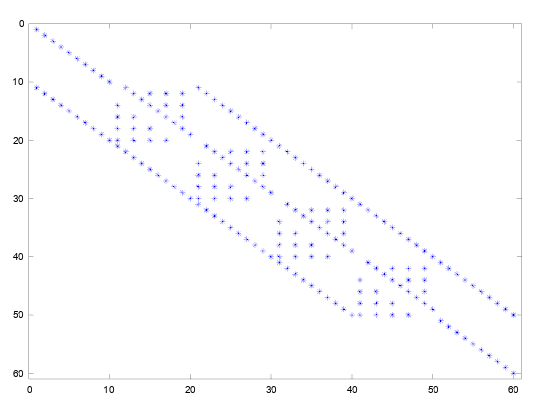
\includegraphics[width=\textwidth]{spy.png}
\caption{spy(A) for model 1 with N = M = 5}
\label{fig:spy}
\end{figure}

\subsection*{Model 2}
This time $u(x, 0) = e^{-3(x-2)^2}$ and $v_0$ is set to $D^{3/2}_xu_0(x)$, the Caputo Fractional Derivative of order $3/2$ of $u_0$. The integral given ($\frac{1}{\Gamma(1/2)}\int_0^x{\frac{u''_0(\hat x)}{\sqrt{x-\hat x}}d\hat x}$) cannot be integrated analytically, but can be approximated numerically; we used the method provided on the web page to do this, where we chose $k = 2M$ (we did try $k = 10M$, but this yielded seemingly identical results, so $k = 2M$ seems to be a safe choice). Plots of the initial conditions on $u$ and $v$ can be seen in figure \ref{fig:2init}. The final condition on $u$ and $v$ are not known analytically now. Let us take a look at the equations to find an estimate.%Chose higher k?

\begin{figure}
\centering
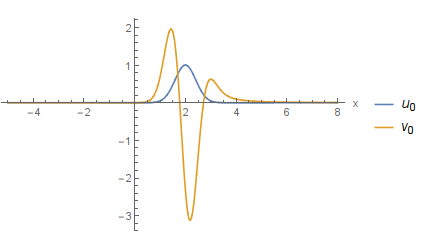
\includegraphics[width=0.7\textwidth]{2init.png}
\caption{The initial conditions for model 2}
\label{fig:2init}
\end{figure}
We do still have:
$$u_{tt} = u_{xxx}$$
And at $t=0$ we have $u_t = v = D^{3/2}_x u$, and $v_t = u_{tt} = u_{xxx} = D^{3/2}_x(D^{3/2}_x u) = D^{3/2}_x v$;
So as long $v = D^{3/2}_x u$ is satisfied we can write our ODEs as;
$$
\begin{cases}
u_t = D^{3/2}_x u\\
v_t = D^{3/2}_x v\\
\end{cases}
$$
%Now we will show that the equation $v = D^{3/2}_x u$ at $t=0$ will hold for other values of $t$ as well.%TODO: does this actually hold?
%$\frac{\partial}{\partial t}(v - D^{3/2}_x u) = v_t - D^{3/2}_x v = u_{xxx} - D^{3/2}_x v$

Under these circumstances we expect $u$ and $v$ to behave ``independently'' according to the same ODE. As a result, we expect that they will keep satisfying these equations for $t\not = 0$ as well. The dynamics should be somewhere in between the advection ($u_t = u_{x}$) and heat ($u_t = u_{xx}$) equation. In the advection equation we expect the initial condition to move to the $-x$ direction with constant speed. In the heat equation we expect a lot of diffusion. Hence for our ``hybrid'' ODE we qualitatively expect some damped movement in the $-x$ direction. If the damping goes fast enough, the ``mass'' in the initial condition will be spread more evenly at $t = 1$. Hence choosing $v = u = 0$ at $t = 1$ seems reasonable (we will verify this choice with a numerical experiment). We expect that the (non-zero part of the) solution will stay away from $x=-5$ and $x=8$ since the initial value is significantly bigger than $0$ for $x\in [0, 6]$ only, leaving a size $5$ buffer to the left and a size $2$ buffer to the right. Hence we choose $v(-5, t) = v(8, t) = 0$. 

Now for our choice of $\dx$. We have $u = v = 0$ for $x = -5$ and $x = 8$, so we want $x_0 = -5 + \dx$ and $x_{M-1} = 8 - \dx$. So we set $x = -5 + (i+1)\dx$ with $\dx = \frac{13}{M+1}$.

\clearpage

\section*{Perform numerical experiments with the BV-technique applied to both models. Illustrate your report with a couple of plots and tables}
\subsection*{Model 1}
In figure \ref{fig:spy}, the position of non-zero elements in our matrix $A$ can be seen.
We tested our method for $N = 10$ and $M = 100$. See figure \ref{fig:ucomp1} through \ref{fig:verr1} for a comparison of the exact solution and the values found with the BV-technique. Our implementation gives a reasonable estimation of $u$ and $v$, but a high accuracy is not achieved, especially when we consider the computational intensity of the BV-method. Also notice that $u$ behaves differently on even and odd time steps (see figure \ref{fig:uerr1}). $u$ is relatively accurate on even time steps, but is split into two different modes on odd time steps, above (for odd $i$) and one below (for even $i$) the exact solution.
Why exactly this is the case is not clear to me, but one can observe that with our choice of discretization we are actually solving two independent systems of equations; $u$ on odd time steps and $v$ on even time steps depend on each other and are independent of $u$ on even time steps and $u$ on odd time steps. Somehow one of these systems was solved nicely while the other developed the strange oscillations in $u$ we observed. We think this has something to do with the initial and final condition imposed on $u$ and $v$. For even values of $N$ we have the following situation:

\begin{center}
\begin{tabular}{c|cc}
$N$ even & $u$ & $v$\\
\hline
0 & $A$ & $B$ \\
1 & $B$ & $A$ \\
2 & $A$ & $B$ \\
$\vdots$ & $\vdots$ & $\vdots$ \\
$N-1$ & $B$ & $A$ \\
$N$ & $A$ & $B$ \\
\end{tabular}
\end{center}

Here $A$ and $B$ are labels for the two independent systems. We have observed that system $B$ somehow develops oscillations in $u$. Perhaps the fact that we only directly impose our initial/final condition on $v$ in system $B$ has something to do with this behavior. We did observe that $A$ and $B$ behave more similarly when $N$ was chosen odd;

\begin{center}
\begin{tabular}{c|cc}
$N$ odd & $u$ & $v$\\
\hline
0 & $A$ & $B$ \\
1 & $B$ & $A$ \\
$\vdots$ & $\vdots$ & $\vdots$ \\
$N-1$ & $A$ & $B$ \\
$N$ & $B$ & $A$ \\
\end{tabular}
\end{center}

Now both systems have one direct constraint on $u$ and one direct constraint on $v$. We have solved a system with $N = 9$ and $M = 100$, this took about $0.3$ seconds. The absolute error in $u$ improved by approximately a factor 3. See figure \ref{fig:uerr1small} and \ref{fig:verr1small}.
We have solved a system with $N = 201$ and $M = 200$, this took about $30$ seconds. See figure \ref{fig:uerr1big} and \ref{fig:verr1big} for the errors.

\begin{figure}
\centering
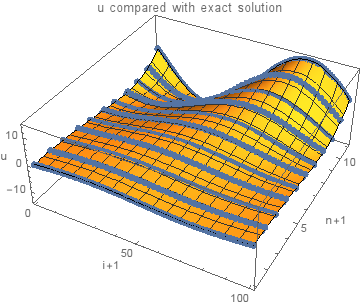
\includegraphics[width=0.6\textwidth]{uCompared.png}
\caption{In this plot the yellow surface represents the exact solution of $u$, while the blue lines are the results from the BV method for Model 1 with $N=10$ and $M=100$}
\label{fig:ucomp1}
\end{figure}

\clearpage

\begin{figure}
\centering
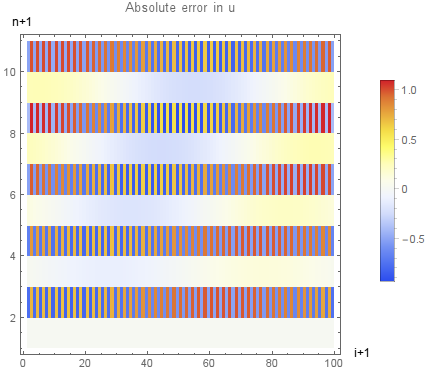
\includegraphics[width=0.6\textwidth]{errorUneat.png}
\caption{The absolute error in $u$ (Model 1 with $N=10$ and $M=100$)\\Notice that the error is low in even time steps, but has higher amplitude (about $10\%$ relative error) and is alternating rapidly on odd time steps.}
\label{fig:uerr1}
\end{figure}

\begin{figure}
\centering
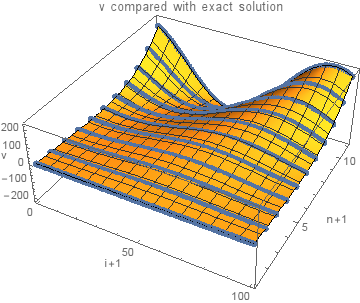
\includegraphics[width=0.6\textwidth]{vCompared.png}
\caption{In this plot the yellow surface represents the exact solution of $v$, while the blue lines are the results from the BV method for Model 1 with $N=10$ and $M=100$}
\label{fig:vcomp1}
\end{figure}

\begin{figure}
\centering
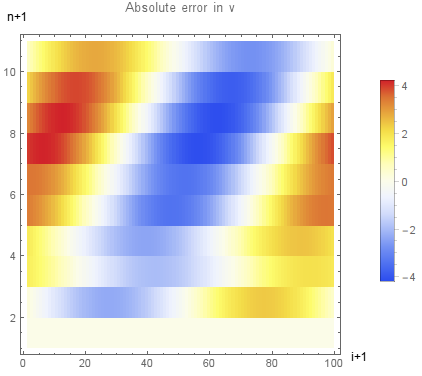
\includegraphics[width=0.6\textwidth]{errorVneat.png}
\caption{The absolute error in $v$ (Model 1 with $N=10$ and $M=100$)\\Notice that the amplitude of these errors is around 4, while the amplitude of $v$ is around 200. }
\label{fig:verr1}
\end{figure}

\begin{figure}
\centering
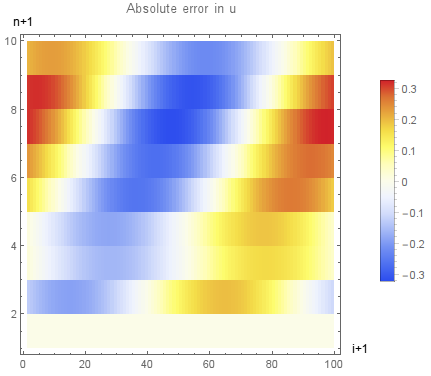
\includegraphics[width=0.6\textwidth]{errorUneat9x100.png}
\caption{The absolute error in $u$ (Model 1 with $N=9$ and $M=200$)\\Notice that the error is much smaller (approximately a factor 3) than that with $N=10$ and $M=200$.}
\label{fig:uerr1small}
\end{figure}

\begin{figure}
\centering
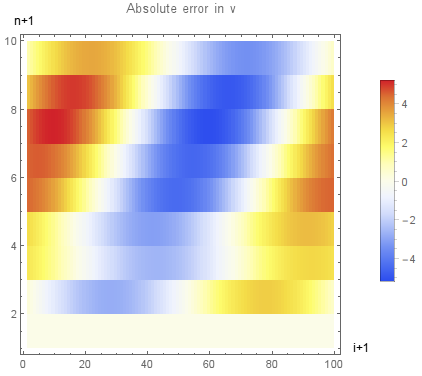
\includegraphics[width=0.6\textwidth]{errorVneat9x100.png}
\caption{The absolute error in $v$ (Model 1 with $N=9$ and $M=200$)\\Notice that the error is similar to that with $N=10$ and $M=200$.}
\label{fig:verr1small}
\end{figure}


\begin{figure}
\centering
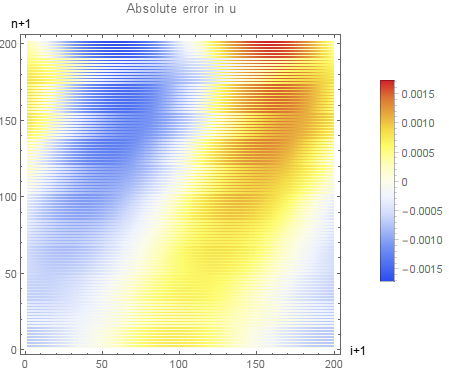
\includegraphics[width=0.6\textwidth]{errorUneat201x200.png}
\caption{The absolute error in $u$ (Model 1 with $N=201$ and $M=200$)\\Notice that the error is quite low.}
\label{fig:uerr1big}
\end{figure}

\begin{figure}
\centering
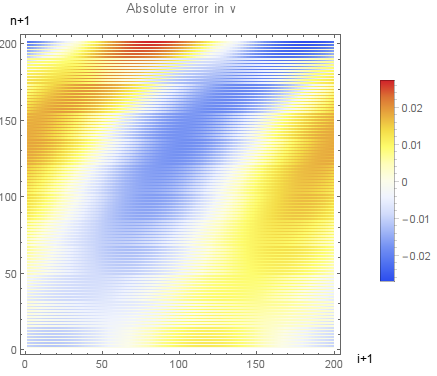
\includegraphics[width=0.6\textwidth]{errorVneat201x200.png}
\caption{The absolute error in $v$ (Model 1 with $N=201$ and $M=200$)\\Notice that the error is quite low.}
\label{fig:verr1big}
\end{figure}

\clearpage

\subsection*{Model 2}
As mentioned before we chose our boundary values ($u = v = 0$ at $x = -5$, $x = 8$ and $t = T$) to be zero, because low values are to be expected after a lot of smoothing has occurred. To numerically verify that the given model will indeed be near zero at $t=1$, we first ran our simulation until $t=10$. The results can be seen in figure \ref{fig:uvdamp}. We noticed small oscillations between even and odd time steps in both $u$ and $v$, although they are not as bad as we observed for even values of $N$. To get a rough estimate of the amplitude of these oscillations, we compared the linear average of two adjacent odd time steps in $u$ with the even time step in between them. The result can be seen in figure \ref{fig:oscsize}. Linear interpolation is not perfect, hence we can see that the curvature of $u$ some effect on this plot; see the small wave near $t=x=0$ (so $i \approx 100$ and $n = 0$), with amplitude about $0.01$. We can also see a big wave at $t=10$ with amplitude $0.05$, where $u$ appears to be nice and flat; this is an estimate of the size of the oscillations in $u$.

\begin{figure}
\centering
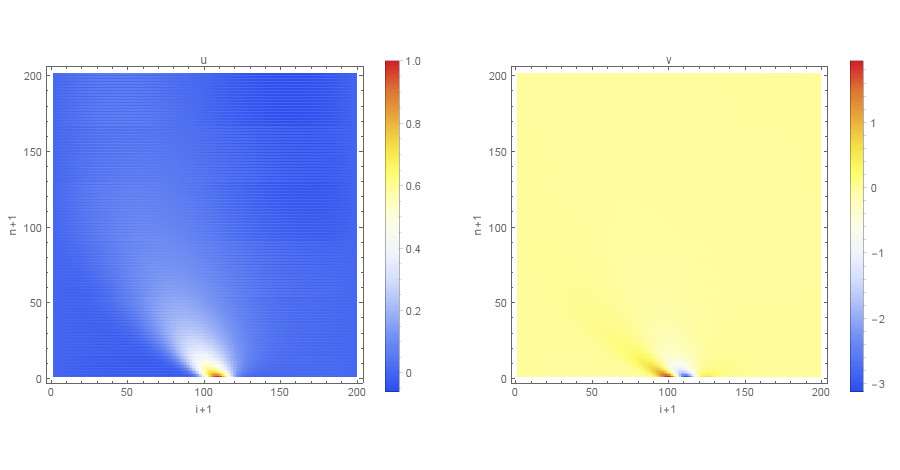
\includegraphics[width=1.1\textwidth]{uvdamping.png}
\caption{$u$ and $v$ for model 2 with $N=201$, $M=200$. Here $t\in[0,10]$, all other parameters are as specified in the exercise. Notice that we do indeed observe damping and a translation in the $-x$ direction for both $u$ and $v$.}
\label{fig:uvdamp}
\end{figure}

\begin{figure}
\centering
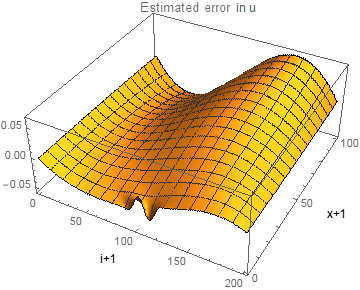
\includegraphics[width=0.5\textwidth]{oscsize.png}
\caption{An estimate of the size of oscillations in $u$.}
\label{fig:oscsize}
\end{figure}

Both $u$ and $v$ are non-zero at $t=1$, but still have peaks with amplitude in the order of $0.2$. While choosing $u = v = 0$ at $t=1$ is no terrible choice, we might be able to do better. We hope that because we let the simulation run until $t=10$ our solution at $t=1$ is largely independent of the final condition. To test this theory, we choose different reasonable constant values for $u$ and $v$ at $t=10$ and compared the solution at $t=1$. See figures \ref{fig:uFinals} and \ref{fig:vFinals}. We see that the solution tends to damp out, so at $t=10$ we would find amplitudes between $0$ and $0.2$ reasonable. We fitted functions through the curves found with value $0$ at $x=-5$ and $x=8$, which we use as final conditions on $u$ and $v$ in our final simulation with $T=1$.

\begin{figure}
\centering
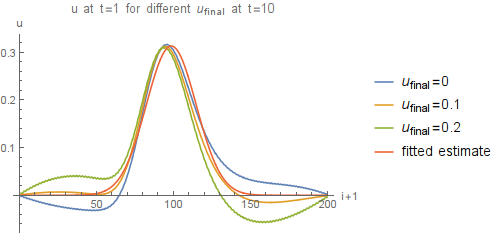
\includegraphics[width=0.6\textwidth]{uFinals.png}
\caption{$u$ at $t=1$ for different $u(x, T) = v(x, T)$. We fitted a Gaussian function. Notice that this function lies within the region of reasonable solutions.}
\label{fig:uFinals}
\end{figure}

\begin{figure}
\centering
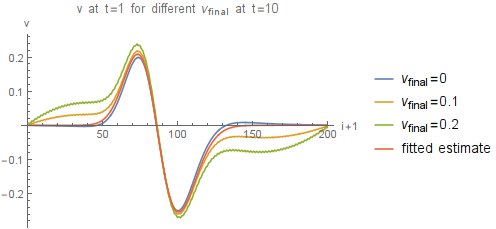
\includegraphics[width=0.6\textwidth]{vFinals.png}
\caption{$v$ at $t=1$ for different $u(x, T) = v(x, T)$. We fitted the sum of two Gaussian functions. Notice that the result lies within the region of reasonable solutions.}
\label{fig:vFinals}
\end{figure}

The result of this simulation can be seen in figure \ref{fig:uvResult}. Notice that it still contains some oscillations, we estimated the amplitude of these oscillations to be around $0.05$ (using the same method as before, see \ref{fig:errorFinal}). Despite these numerical errors, both $u$ and $v$ behave as we expected qualitatively.

\begin{figure}
\centering
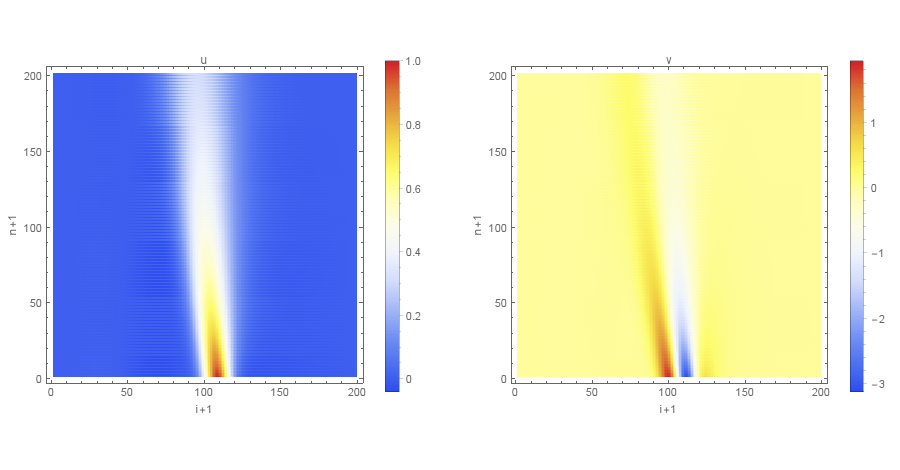
\includegraphics[width=1.0\textwidth]{uvResult.png}
\caption{$u$ and $v$ found with the fitted final condition, using $N=201$ and $M=100$.}
\label{fig:uvResult}
\end{figure}

\begin{figure}
\centering
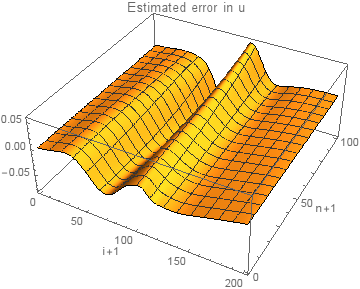
\includegraphics[width=0.5\textwidth]{errorFinal.png}
\caption{Estimate of the amplitude of oscillations in $u$. Notice that this amplitude has size at most 0.05, which is a relative error in the order of $15\%$.}
\label{fig:errorFinal}
\end{figure}

\section*{How would FTCS and BTCS perform when applied to these models?}
Neither can be stable because of their stability region. See the practical part of SC1 for an explanation.

\section*{Appendix A: BV-method implementation for model 1}
\lstinputlisting{bvmodel1.m}

\section*{Appendix B: BV-method implementation for model 2}
\lstinputlisting{bvmodel2.m}


\end{document}

